\chapter{Opis projektnog zadatka}
		{Cilj ovog projekta je napraviti web aplikaciju HGSStracks koja olakšava koordinaciju rada svih ljudi, spasioca ili dispečera, aktivnih na akciji spašavanja. Aplikacija korisniku omogućava praćenje akcije spašavanja osobe prijavljene kao nestale. Također omogućuje nadležnoj osobi koordinaciju spasioca na terenu u stvarnom vremenu. Aplikacija služi kao potpuna postojeće aplikacije napravljene od strane organizacije "Hrvatski Crveni križ"(nadalje u tekstu HCK), koja pruža razne informacije vezane uz spašavanje ljudi, koje je zadesila nesreća, te kako medicinski pomoći osobi ako je potrebno.\\
			\begin{figure}[h!]
				\centering
				\begin{subfigure}[b]{0.3\linewidth}
					\centering
					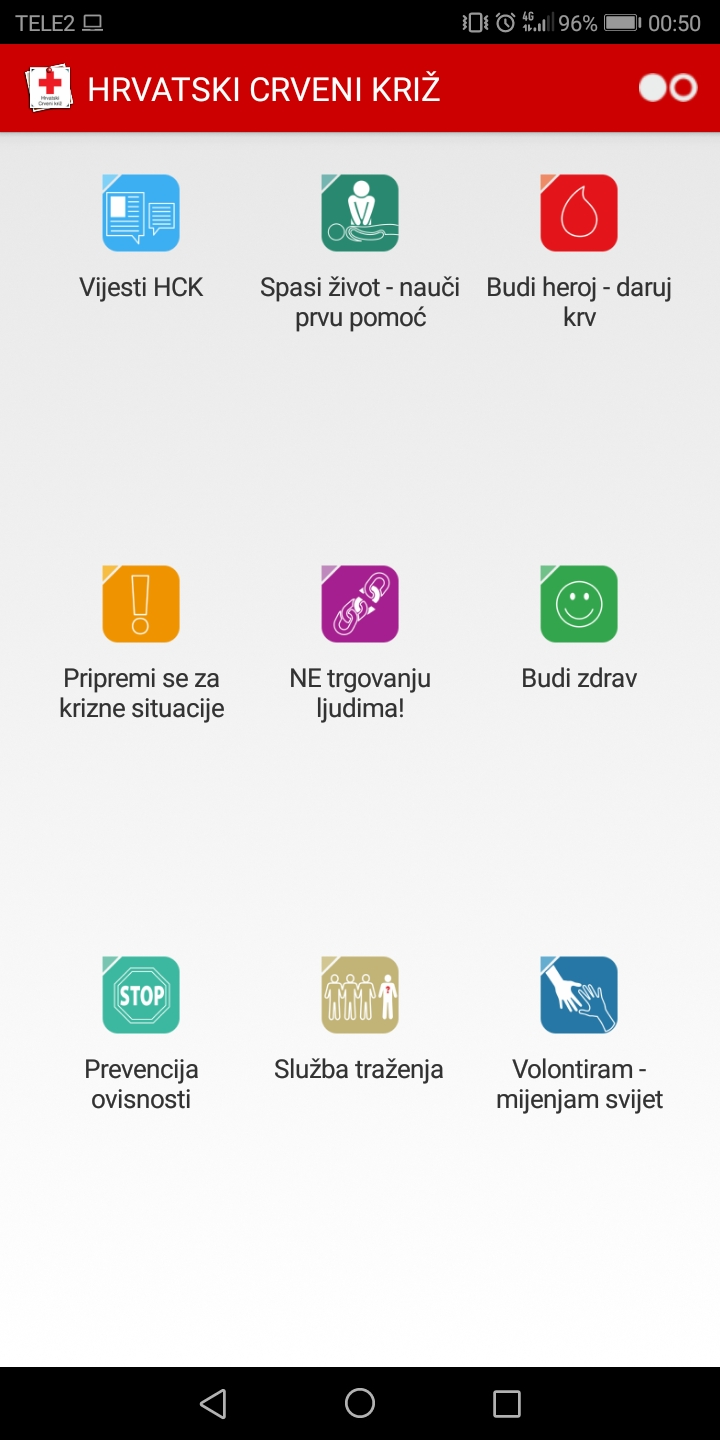
\includegraphics[scale=0.1]{./slike/crv1.jpg}
					\caption{\tiny Početna stranica aplikacije HCK}
					\label{fig:sub-first}
				\end{subfigure}
				\begin{subfigure}[b]{0.3\linewidth}
					\centering
					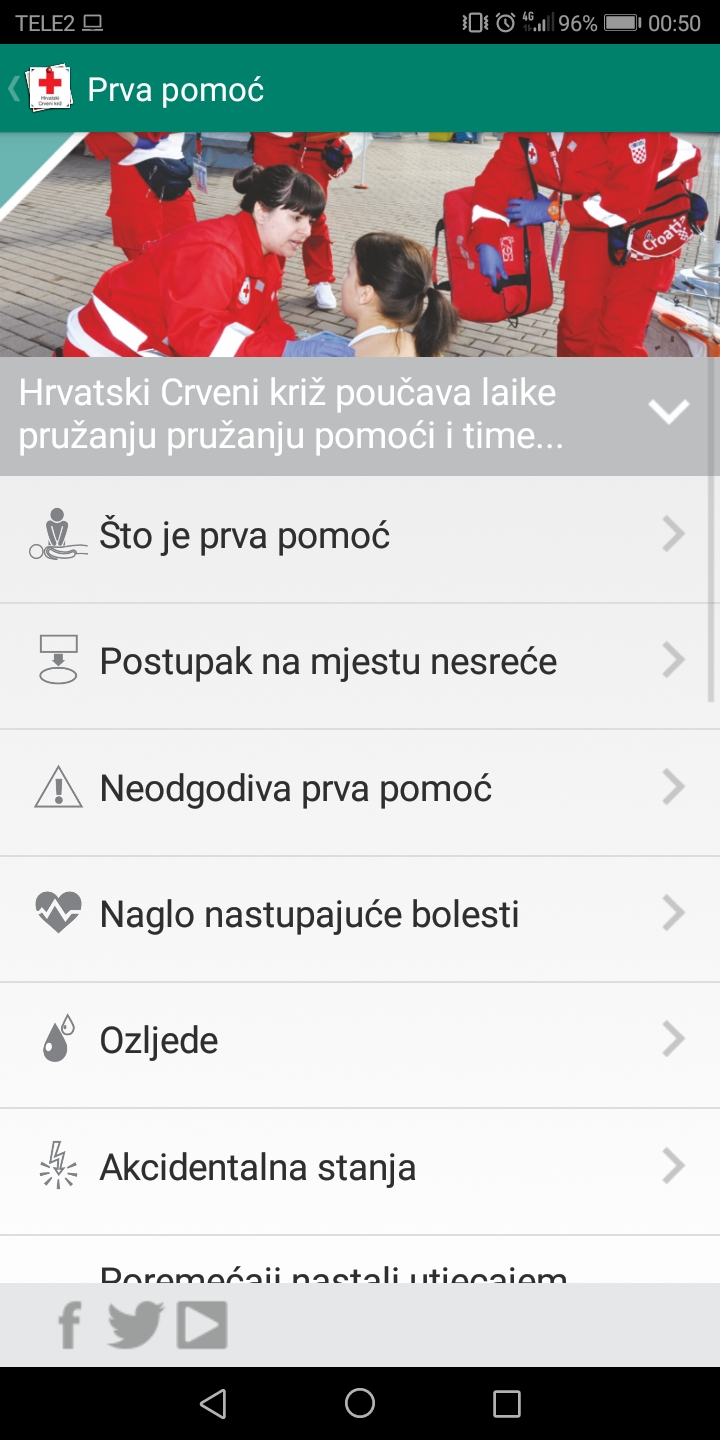
\includegraphics[scale=0.1]{./slike/crv2.jpg}
					\caption{\tiny Podstranica aplikacije HCK s uputama za prvu pomoć}
					\label{fig:sub-second}
				\end{subfigure}
				\begin{subfigure}[b]{0.3\linewidth}
					\centering
					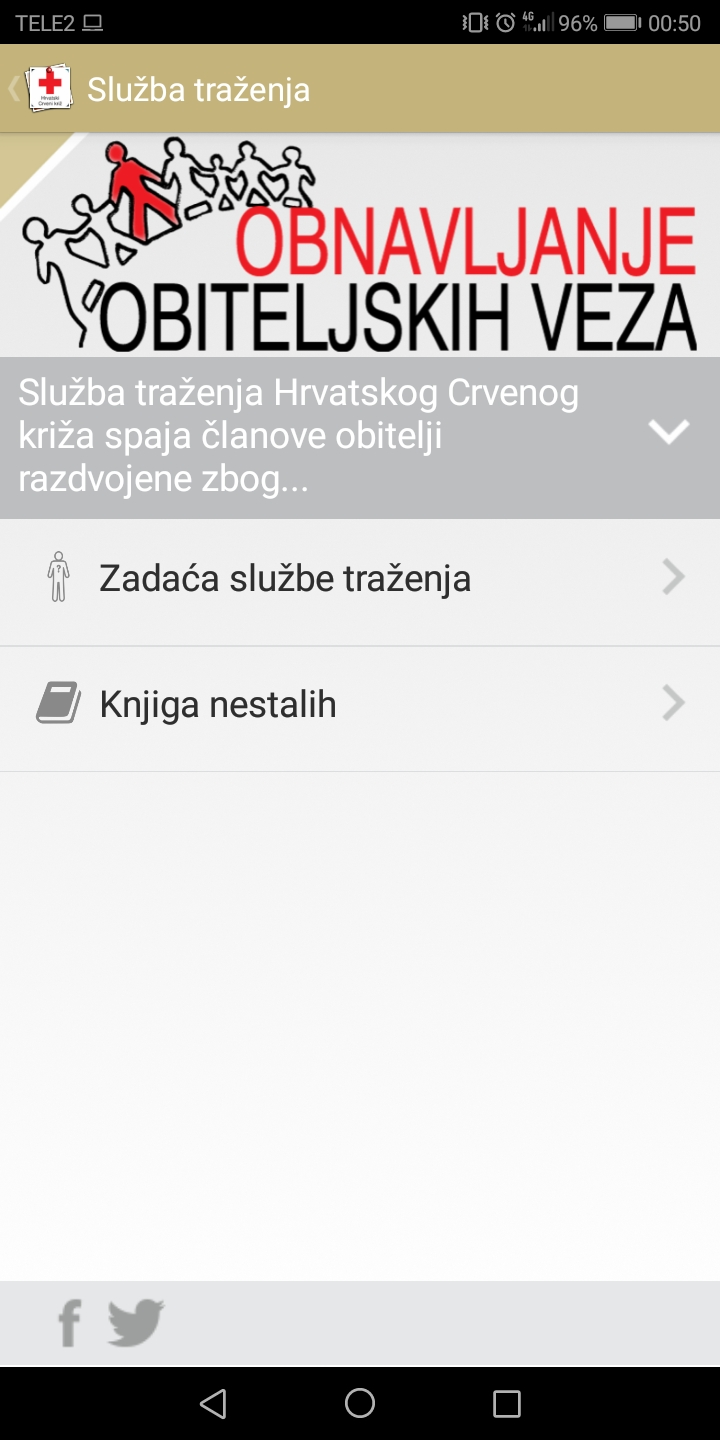
\includegraphics[scale=0.1]{./slike/crv3.jpg}
					\caption{\tiny Podstranica aplikacije HCK s knjigom nestalih te opisom rada službe za spašavanje}
					\label{fig:sub-third}
				\end{subfigure}
			\caption{Prikaz postojeće aplikacije HCK}
			\label{fig:fig}
			\end{figure}\\
			
			Cilj aplikacije je brzo i jednostavno reagiranje na prijavu nesreće ili nestanka osobe, te umanjenje potrebnog vremena za spašavanje žrtava nesreće. Također odvajamo uloge, i zadatke po ulogama, kako bi osobe na terenu znale što su dužne odraditi, gdje trebaju doći i tko je u opasnosti.\\
		Prilikom pokretanja sustava korisnike se pita za autentifikaciju kredencija ako imaju već izrađen i autoriziran račun od strane administratora.\\
		Neregistrirani korisnici mogu se registrirati s postojećim računom ili kreirati novi račun pritiskom na gumb – Registracija. 
		\\\\Za registraciju korisnik bira ulogu koju želi obnašati (spasilac, dispečer) te su potrebni sljedeći podaci:}


		\begin{packed_item}
			\item {korisničko ime} 
			\item {fotografija}
			\item {lozinka}
			\item {ime}
			\item {prezime}
			\item {broj mobitela}
			\item {email adresa}
		\end{packed_item}
	
		{Prilikom registracije korisnika zahtjev se šalje administratoru koji ju je dužan odobriti ili odbiti. Ovisno o ulozi koju je izabrao, te mu je ona odobrena od administratora, registracijom u sustav korisniku se dodjeljuju određena prava ovisno o njegovoj ulozi u aplikaciji.\\
			
			Postoje 4 vrste korisnika popisana silazno prema razini ovlasti koje imaju za vrijeme korištenja aplikacije: Administrator, Dispečer, Voditelj, Spasilac.\\ 
			
			\begin{wrapfigure}{l}{0.25\textwidth}
				\centering
				
\includegraphics[width=0.25\textwidth]{./slike/spasioc.png}
				\caption{Ikona spasioca}
			\end{wrapfigure}
			\textbf{Spasilac} pripada nekoj stanici i redovito je dužan osvježavati podatak o dostupnosti za akcije spašavanja koje je moguće da sam podesi na svojem profilu ili ako je stavljen u akciju spašavanja od strane dispečera automatski je postavljeno u "Nedostupan". Spasilac se sam može odazvati na akciju ako zadovoljava tražene kriterije koje je postavio Dispečer; može potvrditi zahtjev poslan od dispečera ako on smatra da je potreban akciji a on se nije javio na istu.\\ Tijekom akcije na karti ostavlja trag kojim prolazi (trag ostavlja pomoću GPS-a na mobilnom telefonu) i time pokazuje svoj položaj Dispečeru u obliku toplinske karte. Na karti mu se prikazuju zadaci koje treba obaviti zadane od strane Voditelja ili Dispečera, privremene i stalne postaje te trenutna pozicija ostalih spasilaca aktivnih na akciji spašavanja. Spasilac u njegovoj aktivnoj akciji ima mogućnost ostavljanja komentara na ruti kroz koju prolazi za ostale sudionike spašavanja.\\
			
			
			\begin{wrapfigure}{r}{0.25\textwidth}
				\centering
				
\includegraphics[width=0.25\textwidth]{./slike/leader.png}
				\caption{Ikona voditelja spasioca}
			\end{wrapfigure}
			\textbf{Voditelj} spasioca je glavni spasilac u stanici. On je i sam spasilac, no ima specifične ovlasti koje "običan" spasilac nema. Pod posebne ovlasti Voditelja spada definiranje načina na koji su određeni Spasioci vlastite stanice voditelja osposobljeni obavljati akcije spašavanja unesrećene osobe. Ovisno o načinu izvođenja spašavanja spasilac ima definiranu veličinu i intenzitet područja kojeg može u trenu vidjeti na karti u aplikaciji.\\
			Vrste izvođenja spašavanja su:
			
			\begin{packed_item}
				\item {Auto} 
				\item {Bicikl}
				\item {Pješice}
				\item {Pas}
				\item {Dron}
				\item {Helikopter}
				\item {Plovilo}
			\end{packed_item}
		
		
			\begin{wrapfigure}{l}{0.25\textwidth}
				\centering
				
\includegraphics[width=0.25\textwidth]{./slike/Dispatch.png}
				\caption{Ikona dispečera}
			\end{wrapfigure}
			\textbf{Dispečer} je osoba odgovorna za raspoređivanje osoblja i nadziranja rada cijelog sustava akcija spašavanja osoba iz jednog centriranog odjela udaljenog od samih akcija.Slijedno dostavi prijave nesreće,dužan je otvoriti akciju spašavanja s informacijama o nestaloj osobi, te nakon što je osoba pronađena i pružena joj je potrebna pomoć završava akciju te je sprema u bazu "riješenih" akcija. Početkom akcije ima uvid u broj dostupnih spasilaca po stanicama u blizini nestanka osobe te ima mogućnost poslati zahtjev za uključivanje spasilaca u akciju,i ako procjenom zaključi da je potreban veći broj spasioca može dodati spasioce iz udaljenih stanica, te ih može ukloniti s akcije u slučaju njihovih upitnih postupaka za vrijeme spašavanja. Prilikom slanja zahtijeva, dispečer definira način sudjelovanja spasilaca (ako postoji mogućnost u stanici gdje je spasilac stacioniran), zadaje im individualne zadatke te ima mogućnost postavljanja dodatnih komentara za zadate ; izbjegavanje određenih stvari, moguće alergije na penicilin itd. \\ Mogući zadatci su:
			
			\begin{packed_item}
				\item {Prođi određenom rutom} 
				\item {Postavi privremenu postaju}
				\item {Osvježi zalihe u privremenoj postaji}
				\item {I sl.}
			\end{packed_item}
			
			Uz zadatke zadane spasiocima na karti prikazuju mu se i tragovi svih aktivnih spasioca unutar zadnja 2 sata. Dispečer ima mogućnost uključivanja prikaza toplinske karte temeljene na dosadašnjim prijeđenim tragovima spasioca i načinima na koje sudjeluju(navedenim u paragrafu Voditelja spasioca).\\
		
			\textbf{Administrator} može vidjeti popis svih registriranih korisnika sustava te njihove osobne podatke, izmjenjivati dodijeljena prava i određene podatke. U slučaju zatražene registracije vrši provjeru kredencija mogućeg novog korisnika te je potvrđuje, i dodjeljuje potrebne ovlasti ako su one odobrene od strane samog HGSS-a; Voditelj, Dispečer, Spasilac. \\ Jedan od zadataka administratora je pregled podataka i njihove točnosti u samom sustavu te izrada sigurnosne kopije na udaljenom mjestu za slučaj pada samog sustava. U slučaju trajnog zatvaranja tj. otvaranja stanice na karti dužan je podatke korigirati u sustavu tj. bazi. U slučaju pada sustava administrator pregledava razlog istog, te nakon otklanjanja problema ponovno pokreće sustav i ažurira podatke ovisno o promjenama do kojih je došlo između pada i ponovnog pokretanja sustava.\\}\\*
		
		